\documentclass[a4paper, 11pt]{article}
\usepackage[english]{babel}
\usepackage[utf8]{inputenc}
\usepackage{amsmath}
\usepackage{graphicx}
\usepackage{float}
\usepackage{fixltx2e}
\usepackage{listings}
\usepackage{color}
\usepackage{latexsym}
\usepackage{lstautogobble}
\usepackage[colorinlistoftodos]{todonotes}
\usepackage[margin=3cm]{geometry}
\usepackage{hyperref}
\usepackage{libertine}
\usepackage{tikz}
\hypersetup{
	hidelinks, 
	colorlinks = true,
	linkcolor = black,
}

\usetikzlibrary{shapes, arrows}

\newtheorem{definit}{Definizione}[subsection]
\newcommand{\encr}{E_e}
\newcommand{\decr}{D_d}

\begin{document}
	\clearpage
	\begin{titlepage}
		\centering
		\vspace*{\fill}
		{\scshape\LARGE Università degli Studi di Verona \par}
		\vspace{1.5cm}
		\line(1,0){230} \\
		{\huge\bfseries Sicurezza delle reti\par}
		\line(1,0){230} \\
		\vspace{0.5cm}
		{\scshape\Large Riassunto dei principali argomenti\par}
		\vspace{2cm}
		{\Large\itshape Davide Bianchi\par}
		\vspace{1cm}
		\vspace{5cm}
		\vspace*{\fill}
		% Bottom of the page
		{\large \today\par}
	\end{titlepage}
	\thispagestyle{empty}
	\newpage
	\tableofcontents
	\newpage
	
	\section{Introduzione}
	
	\begin{definit}[Information Security]
		Protezione delle informazioni e dei sistemi per impedirne l'accesso non autorizzato, uso, divulgazione, modifica o distruzione.
	\end{definit}
	
	\begin{definit}[Network Security]
		Protezione dell'accesso a risorse situate all'interno di una rete.
	\end{definit}
	
	Nella sicurezza si distinguono una \textbf{policy}, un \textbf{meccanismo} e una \textbf{compliance}.
	Una security policy specifica il comportamento che il sistema può o non può assumere. I meccanismi di sicurezza sono l'implementazione di una data policy. Diciamo quindi che una security policy $\phi$ deve rimanere valida per un sistema $P$ in ogni ambiente malevolo $E$, ovvero $P \parallel E \models \phi $.
	
	Le politiche di sicurezza sono spesso formulate per arrivare ad alcune proprietà standard, le più comuni sono:\begin{itemize}
		\item Confidenzialità: non ci sono fughe di informazioni;
		\item Integrità: non ci sono modifiche alle informazioni;
		\item Disponibilità: non ci sono "danneggiamenti" ai servizi;
		\item Accountability\footnote{La traduzione più vicina è \textit{responsabilità}.}: le azioni sono sempre riconducibili ai diretti responsabili;
		\item Autenticazione: l'origine dei dati può essere identificata con sicurezza.
	\end{itemize}
	
	\paragraph{Contromisure per la protezione.} Le principali tecniche di contromisura consistono in:\begin{itemize}
		\item Prevenzione di breach;
		\item Rilevamento di attacchi in corso;
		\item Reazione ad un possibile attacco.
		\end{itemize}
		
	\section{Cenni di crittografia}
	\subsection{Introduzione}
	Iniziamo dando alcune definizioni fondamentali. Si useranno i termini \textit{ciphertext} e \textit{plaintext} per indicare rispettivamente il testo cifrato e quello in chiaro.
	
	\begin{definit}[Crittografia]
	Insieme dei metodi per rendere un messaggio non leggibile ad altri.
	\end{definit}
	
	\begin{definit}[Steganografia]
	Insieme dei metodi per nascondere l'esistenza di un messaggio in un altro contenuto.
	\end{definit}
	
	\begin{definit}[Crittoanalisi]
	Analisi del ciphertext per ottenere il plaintext corrispondente.
	\end{definit}
					
	Un generico sistema crittografico è strutturato come: \\
	
	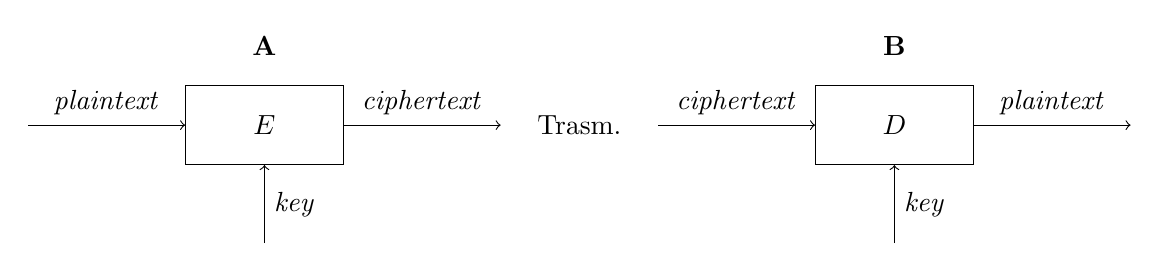
\begin{tikzpicture}
	\node at (4,0) [rectangle,draw, minimum width=2cm, minimum height=1cm] (E) {$E$};
	\draw (E);
	\draw[->] (1,0) -- (E) node[above, midway] {\textit{plaintext}};
	\draw[->] (4,-1.5) -- (E) node[right, midway] {\textit{key}};
	\draw[->] (E) -- (7,0) node[above, midway] {\textit{ciphertext}};
	\node at (8,0) (dots) {Trasm.};
	\node at (12,0) [rectangle,draw, minimum width=2cm, minimum height=1cm] (D) {$D$};
	\draw[->] (9,0) -- (D) node[above, midway] {\textit{ciphertext}};
	\draw[->] (12,-1.5) -- (D) node[right, midway] {\textit{key}};
	\draw[->] (D) -- (15,0) node[above, midway] {\textit{plaintext}};
	\node at (4,1) {\textbf{A}};
	\node at (12,1) {\textbf{B}};
	\end{tikzpicture}
	
	In crittografia si distinguono le due categorie \textit{a chiave simmetrica} e \textit{a chiave asimmetrica}. La differenza sta nel fatto che nella crittografia a chiave simmetrica le due entità che si scambiano il messaggio devono condividere una stessa chiave (che deve essere trasmessa su un canale sicuro), mentre nella crittografia a chiave asimmetrica le chiavi sono differenti e sono 2 per ogni entità, una pubblica e una privata. Nella crittografia a chiave asimmetrica si elimina il problema della condivisione della chiave; inoltre la chiave pubblica può essere compromessa da attaccanti senza che la chiave privata venga compromessa, e senza che venga compromessa la segretezza del messaggio.
	
	Un altro aspetto fondamentale della crittografia è che la cifratura e la decodifica sono facili, \textit{se le chiavi sono note}. Da ciò consegue che la sicurezza debba risiedere nella chiave, non nell'algoritmo in se.
	
	\subsection{Crittoanalisi}
	La scienza di recuperare il messaggio in chiaro senza conoscere il ciphertext si basa sostanzialmente su due differenti approcci:
	\begin{itemize}
		\item attacco brute-force;
		\item attacco crittoanalitico.
	\end{itemize}
	
	\paragraph{Attacco brute-force.} Un attacco bruteforce è semplice: consiste nel provare tutte le chavi possibili fino ad indovinare quella corretta. Questa tipologia di attacco in generale è sempre possibile nella sua semplicità, tuttavia, se la dimensione dello spazio delle chiavi inizia ad essere elevata, il tempo che si deve impiegare diventa insostenibile, per cui in questi casi è necessario ricorrere ad altri stratagemmi.
	
	\paragraph{Attacco crittoanalitico.} In questo caso si assume che l'attaccante conosca l'algoritmo utilizzato nella cifratura dei messaggi; si trova quindi una qualche debolezza nell'algoritmo che permetta di farlo fallire. 
	
	In tal senso, si tende a rendere noto un algoritmo affinchè il maggior numero di persone tenti di attaccarlo, per aumentare al massimo le possibilità che venga trovata una falla. (In contrasto con la cosiddetta \textbf{security by obscurity}).
	
	\paragraph{Tipologie di attacco.}Consideriamo ora i possibili attacchi che un sistema crittografico deve affrontare per essere affidabile:
	\begin{itemize}
		\item \textit{known cypertext attack:} questo attaccante è il meno aggressivo e conosce solamente il testo cifrato;
		
		\item \textit{known plaintext attack:} conosce entrambi i tipi di testo;
		
		\item \textit{choosen plaintext:} può scegliere il plaintext da codificare e analizzare il ciphertext ottenuto;
		
		\item \textit{adaptive choosen plaintext:} può liberamente scegliere il plaintext da far codificare e comportarsi di conseguenza, sulla base del risultato appena ottenuto.
		
		\item \textit{chosen ciphertext:} l'attaccante può scegliere differenti ciphertext e avere accesso al plaintext decriptato, per infine ricavare la chiave.
		\end{itemize}
	
	\subsection{Notazione}
	La notazione usata è la seguente: \begin{itemize}
		\item $\mathcal{A}$ è l'alfabeto, ovvero un insieme finito di simboli;
		\item $\mathcal{M} \subseteq \mathcal{A}^*\star$ è il messaggio, dove $M \in \mathcal{M}$ è il \textit{plaintext};
		\item $\mathcal{C}$ è il messaggio cifrato, il cui alfabeto può anche differire da quello usato per $M$;
		\item $\mathcal{K}$ indica lo spazio delle chiavi;
		\item ogni $e \in \mathcal{K}$ denota una funzione biiettiva da $\mathcal{M}$ a $\mathcal{C}$, viene indicata con $\encr$ ed è la funzione di cifratura;
		\item ogni $d \in \mathcal{K}$ è una funzione biiettiva da $\mathcal{C}$ a $\mathcal{M}$, indicata con $\decr$ ed è la funzione di decodifica.
	\end{itemize}

	Data la notazione soprastante, indichiamo con cifrario un insieme $\lbrace \encr\ |\ e \in \mathcal{K} \rbrace$ e il suo corrispondente $\lbrace \decr\ |\ d \in \mathcal{K} \rbrace$ tale che per ogni $e \in \mathcal{K}$ esiste un solo $d \in \mathcal{K}$, in modo tale che $\decr = \encr^{-1}$. La coppia $\langle e, d \rangle$ forma una coppia di chiavi, dove $e$ e $d$ possono anche essere identiche (come nel caso della crittografia simmetrica).
	
	\subsection{Crittografia a chiave simmetrica}
	È il caso più classico. In questo sistema $e = d$, e i due interlocutori condividono una chiave. I cifrari possibili nel caso della crittografia simmetrica sono di 3 categorie: \begin{itemize}
		\item \textit{cifrari a blocchi:} dividono il testo in blocchi di lunghezza fissa e cifrano un blocco alla volta;
		\item \textit{cifrari a flusso:} cifrari a blocchi in cui la dimensione di ogni blocco è fissata a 1;
		\item \textit{codes:} cifrari che lavorano su parole a lunghezza variabile.
	\end{itemize}

	\subsubsection{Tecniche di sostituzione}
	Sono tutti quei cifrari che sostituiscono una lettera con un'altra lettere, basandosi su una qualche regola di sostituzione, come il cifrario di Cesare e la permutazione casuale.
	
	\paragraph{Cifrario di Cesare.}
	Il messaggio viene cifrato sostituendo ogni lettera $l$ del messaggio con la $l+k$ esima lettera dell'alfabeto; la chiave quindi è data dalla coppia $(l, l+k)$. 
	
	Il cifrario di Cesare è facile da attaccare in quanto basta un attacco \textit{bruteforce}, quindi è sufficiente provare tutte le combinazioni (che sono in totale 26).
	
	\paragraph{Permutazione casuale.}
	Supponiamo di usare come cifrario una permutazione casuale dell'alfabeto, ovvero sostituendo ad ogni lettera dell'alfabeto un'altra lettera, in modo totalmente casuale. In tal caso l'attacco bruteforce richiederebbe tempo eccessivo (ci sono $26!$ pssibili combinazioni da provare, che sono decisamente troppe). 
	
	La tecnica usata per attaccare questo tipo di crittografia è l'\textit{analisi delle frequenze}, ovvero l'analisi delle lettere che capitano di più in una data lingua, e associare la lettera del messaggio cifrato con una data frequenza con quella nella lingua del messaggio con una frequenza simile.
	
	\paragraph{Cifrario di Vigenère.}
	Il cifrario di Vigenère riprende l'idea del cifrario di Cesare. L'idea è la seguente: presa una chiave (es. \textit{key}), si ripete la chiave tante volte quanto è lungo il testo (eventualmente troncando l'ultima ripetizione), e si codifica la lettera con il corrispondete cifrario di Cesare. \\
	
	\noindent
	K E Y K E Y K E Y K E Y \\
	P R O V A D I T E S T O \\
	
	
	La prima lettera del cipher text sarà la lettera ottenuta dal cifrario di Cesare di chiave $(K,P)$, la seconda con la chiave $(E, R)$ e così via.
	
	Anche questo cifrario è semplice da attaccare, si parte dalla divisione del ciphertext in gruppi di lunghezza pari a quella della chiave, e si esegue l'analisi delle frequenze su ogni gruppo.
	
	\subsection{Cifrari a trasposizione}
	Funzionano in maniera leggermente diversa. Dato un blocco di lunghezza $l$ e $\mathcal{K}$ un insieme di permutazioni su $\lbrace 1 \dots t \rbrace$, si ha che \[ \encr(m) = m_{e(1)}, \dots, m_{e(2)} \] Per decodificare si applica la permutazione inversa ad ogni carattere del ciphertext.
	
	\subsection{Cifrario di Feistel}
	
	\subsection{Data Encryption Standard (DES)}
	È un cifrario a blocchi che lavora su blocchi di 64 bit. Fu in effetti il primo standard di crittografia, e ne furono rilasciate versioni aggiornate che lavorassero su chiavi di lunghezza maggiore (3-DES). Non è ancora stato violato, ma è possibile ridurre in tempo lineare lo spazio delle chiavi da $2^{56}$ a $2^{43}$.
	
	\begin{center}
		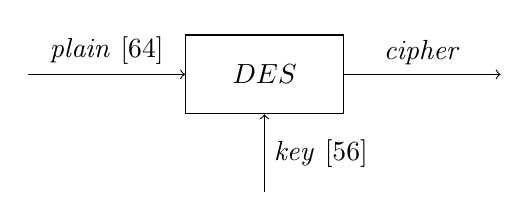
\begin{tikzpicture}
		\node at (4,0) [rectangle,draw, minimum width=2cm, minimum height=1cm] (E) {$DES$};
		\draw (E);
		\draw[->] (1,0) -- (E) node[above, midway] {\textit{plain} $\left[ 64 \right]$};
		\draw[->] (4,-1.5) -- (E) node[right, midway] {\textit{key} $\left[ 56 \right]$};
		\draw[->] (E) -- (7,0) node[above, midway] {\textit{cipher}};
		\end{tikzpicture}
	\end{center}
	
	\subsubsection{Double DES e 3-DES}
	La variante DD, che usa DES due volte consecutive, è soggetta ad un attacco del tipo \textit{Meet-in-the-Middle}.
	\begin{center}
		\begin{tikzpicture}
		\node at (4,0) [rectangle,draw, minimum width=2cm, minimum height=1cm] (E) {$DES$};
		\draw (E);
		\draw[->] (1,0) -- (E) node[above, midway] { $P_1$};
		\draw[->] (4,-1.5) -- (E) node[right, midway] {$K_1$};
		\draw[->] (E) -- (7,0) node[above, midway] {$M$};
		\node at (8,0) [rectangle,draw, minimum width=2cm, minimum height=1cm] (2E) {$DES$};
		\draw[->] (8,-1.5) -- (2E) node[right, midway] {$K_2$};
		\draw[->] (2E) -- (11,0) node[above, midway] { $P_2$};
		\end{tikzpicture}
	\end{center}

	L'attacco funziona nel seguente modo: \begin{enumerate}
		\item Dato un $C = E_{K_2}(E_{K_1}(P))$, sia $X = E_{K_1}(P) = D_{K_2}(C)$;
		\item Dati $P$ e $C$, cifrare $P$ per ogni possibile chiave (sono $2^{56}$);
		\item Generare una tabella con tutti i risultati, ordinati secondo $X$;
		\item Decifrare $C$ con tutte le possibili $K_2$, cercando un matching con quelle i risultati ottenuti prima. Ogni coppia è una possibile coppia valida, basta confrontare i risultati con $P$ e $C$ iniziali.
	\end{enumerate}

	In effetti, guardando lo schema sopra, si nota che al massimo occorrono $2^{56}$ operazioni per violare questo protocollo.
	
	Con 3-DES invece, un tentativo con la soluzione bruteforce necessita di almeno $2^{112}$ operazioni, un numero notevolmente più alto. Al momento infatti non esistono soluzioni per violare 3-DES.
	
	\subsection{Advanced Encryption Standard (AES)}
	Proposto come rimpiazzo di DES nel 1991, fu selezionato nel 2001. Infatti il DES iniziava a non andare più bene, in larga parte perchè era disegnato per i software degli anni 70 ed era abbastanza lento. AES funziona in maniera più snella e lavora su chiavi molto più lunghe (128, 192 e 256 bit).
	
	
	
	
	
	
	
	
	
	
	
	
	
	
	
	

\end{document}